\documentclass{l4dc2027}
% Paper B — L4DC 2027, revision 1 (round-1 panel roadmap docs/paper_b/review/editorial_decision.md;
% facts docs/paper_b/review/revision_facts_2026-11-03.md; response docs/paper_b/review/response_round1.md).
% v1 kept at draft/v1_round1/. Experiments are numbered in reading order; supplement Table S5 maps them to v1's numbers.
\usepackage{times}
\usepackage{booktabs}
\usepackage{array}
\usepackage{siunitx}
\usepackage{tikz}
\usetikzlibrary{positioning,arrows.meta}
\definecolor{lawc}{HTML}{3d5a80}
\definecolor{headc}{HTML}{e0a526}

\makeatletter
\@ifundefined{proposition}{\newtheorem{proposition}{Proposition}}{}
\@ifundefined{lemma}{\newtheorem{lemma}{Lemma}}{}
\@ifundefined{remark}{\newtheorem{remark}{Remark}}{}
\makeatother
\newcommand{\vmax}{v_{\max}}
\newcommand{\wmax}{\omega_{\max}}
\newcommand{\adm}{\mathcal{U}}
\newcommand{\Base}{\textsc{Base}}
\newcommand{\Obs}{\textsc{Obs}}
\newcommand{\Hor}{\textsc{Hor}}
\newcommand{\ObsHor}{\textsc{ObsHor}}
\newcommand{\Free}{\textsc{Free}}
\newcommand{\Aware}{\textsc{Aware}}
\graphicspath{{../figures/}}
\setlength{\textfloatsep}{7pt plus 2pt minus 2pt}
\setlength{\floatsep}{5pt plus 2pt minus 2pt}
\setlength{\intextsep}{7pt plus 2pt minus 2pt}
\setlength{\abovecaptionskip}{4pt}
\setlength{\belowcaptionskip}{0pt}

\title[Safe and Stuck]{The Guarantee Holds and the Task Fails: Absorbing Stalls of Learning-Enabled Controllers under CBF Filters}

\author{%
 \Name{Mohammad Shoaib} \Email{[to confirm]}\\
 \addr NSU Intelligent Robotics Lab, North South University, Dhaka, Bangladesh
 \AND
 \Name{Shahnewaz Siddique} \Email{shahnewaz.siddique@northsouth.edu}\\
 \addr Department of Electrical and Computer Engineering, North South University, Dhaka, Bangladesh%
}

\begin{document}

\maketitle

\begin{abstract}%
A safety filter replaces an unsafe command with the nearest safe one; its guarantee says nothing about the task. We study a pursuit robot whose controller combines a scripted intercept law with a learned search policy, behind a control barrier function (CBF) filter, and find a silent failure: the controller asks to drive into an obstacle or a wall, the filter turns the request into a standstill, the observation stops changing, and the request repeats for the rest of the episode. Collisions are zero and the task fails. At every one of 262 sampled stalled states a turn would have freed the robot. Who keeps asking depends on the controller: against a learned attacker, the scripted law owns 87\% of deadlock episodes in policies trained behind the filter, and the learned head owns 76\% in a policy trained without it; where the head is stuck, escaping is worth at least 0.18 in discounted return, a signal learning does not use. Across ten pre-registered experiments, observation features and a longer horizon raise capture without removing the stall, and two penalties improve a stall metric while capture falls. A one-counter recovery that offers the filter forward and turning commands after $N$ still steps keeps deadlock at or below 0.022 for $N \le 20$ and raises capture on all eleven policies tested, with zero collisions and on a second filter.%
\end{abstract}

\begin{keywords}%
safety filters; control barrier functions; deadlock; liveness; safe reinforcement learning; pursuit--evasion%
\end{keywords}

\section{Introduction}\label{sec:intro}

Safety filters let learned controllers run on robots without collisions. A CBF filter, a shield or a predictive filter checks each command the controller proposes and, if the command is unsafe, executes the nearest safe command instead \citep{hsu2024safetyfilter,ames2019cbf,alshiekh2018shielding,cheng2019endtoend}. The guarantee is that the robot never leaves the safe set. It says nothing about the task.

Figure~\ref{fig:game} shows what can go wrong. A pursuer must catch a faster evader in an arena with obstacles. Its controller was trained without a filter; at deployment a CBF filter is placed in front of it. In panel~(a) the pursuer starts facing a wall and asks to drive forward. The filter allows only standing still or turning, so it stops the pursuer. Nothing the pursuer sees changes, so it asks for the same thing again, at every one of the next 1\,192 steps. The evader is never caught and no collision occurs. In panel~(b), the same episode with a small addition to the filter: after 20 steps without motion, the filter tries driving forward, then turning. The pursuer turns, leaves the wall and catches the evader. Panel~(c) shows the commanded and executed speed.

This failure is easy to miss. The safety record is perfect, the controller is busy, and an average return hides it. We call it an \emph{absorbing stall}: the filter's output and the controller's frozen input form a fixed point of the closed loop. It is related to the deadlocks that CBF quadratic programs create between robots \citep{grover2020symmetry,grover2021deadlock,grover2023before} and to the undesired equilibria they create for a single robot under a fixed nominal controller \citep{reis2021cbfqp,tan2024undesired}. What is new here is what the controller contributes. A controller that includes learning reaches the same fixed point from either of its parts, and learning does not take it out.

\paragraph{Contributions.}
(C1)~The geometry of the stall, measured on 262 stalled states: almost every stall is a trap of the pair (controller, filter) at the current heading, none is a trap of the position, and a turn is always allowed (Lemma~\ref{lem:kkt}, Proposition~\ref{prop:fixed}, Experiment~2).
(C2)~Which part of a learning-enabled controller owns the stall, and why learning does not remove it. In policies trained behind the filter, the scripted law owns most deadlock episodes, inside a single learner decision. In a policy trained without the filter, the learned head owns most. Where the head owns it, the escape carries a large reward signal that learning does not exploit (Experiments~3 and~4).
(C3)~A pre-registered comparison of remedies. Learned remedies improve the task but do not remove the stall, and two penalties make the task worse while a stall metric improves. A one-counter recovery removes the stall with the filter's guarantee untouched, on six policies, over a sweep of its parameter, against a random-perturbation baseline and on a second filter (Proposition~\ref{prop:recovery}, Experiments~5--9).

\section{Related work}\label{sec:related}

\paragraph{Deadlock and undesired equilibria under CBF filters.} \citet{grover2020symmetry,grover2021deadlock,grover2023before} characterise multi-robot deadlock under CBF quadratic programs through the Karush--Kuhn--Tucker (KKT) conditions: the filtered command is zero when the nominal command lies in the cone of the active constraint normals. \citet{reis2021cbfqp} showed that CLF--CBF programs create spurious stable equilibria for one robot; \citet{tan2024undesired} characterised all closed-loop equilibria and removed the undesired ones inside the program, the untested alternative to our recovery; \citet{reis2026stability,reis2025unified} note that liveness is not guaranteed. These works study a fixed nominal controller; we study what a learning-enabled nominal adds.

\paragraph{Shields, liveness and recovery.} \citet{kim2025realizable} require that a continuous-space shield always has a safe action, and note that the shield alone is conservative; \citet{dawood2025dynamic} adapt an MPC shield with a learned supervisor; \citet{wang2025neurosymbolic} resolve multi-robot deadlocks after they occur; \citet{arnstrom2025stealthy} study adversarial filter deactivation.

\paragraph{Learning through the filter.} \citet{oh2026provably} show that a filter-unaware policy chatters against the filter and that training through it is optimal when the filter is permissive enough; \citet{wu2026competence} train game policies through a filter; \citet{georgescu2026gr1} repair a shield's specification online to keep liveness achievable; \citet{pizarro2025filtering} penalise the filter's correction during training. We report a case in which training through the filter, with its state observed, leaves the stall in place.

\section{The game, the controller and the filter}\label{sec:setting}

\paragraph{Game.} A pursuer and an evader move as unicycles in a $10 \times \SI{10}{m}$ arena with two disc obstacles of random radius (0.3--\SI{1.0}{m}) and position in each episode. The pursuer's speed is $v \le \vmax = \SI{1}{m/s}$ and its turn rate $|\omega| \le \wmax = \SI{2.84}{rad/s}$; the evader is 1.2 times faster. One step is \SI{0.05}{s}; an episode ends with a capture (centres within \SI{0.30}{m}) or after 1\,200 steps (a timeout). Each agent sees the other only inside a $90^\circ$, \SI{8}{m} field of view with line of sight not blocked by an obstacle. The evaders are a greedy flee policy, a wall-hugging policy and a learned attacker trained to stall filtered pursuers.

\begin{figure}[t]
\centering
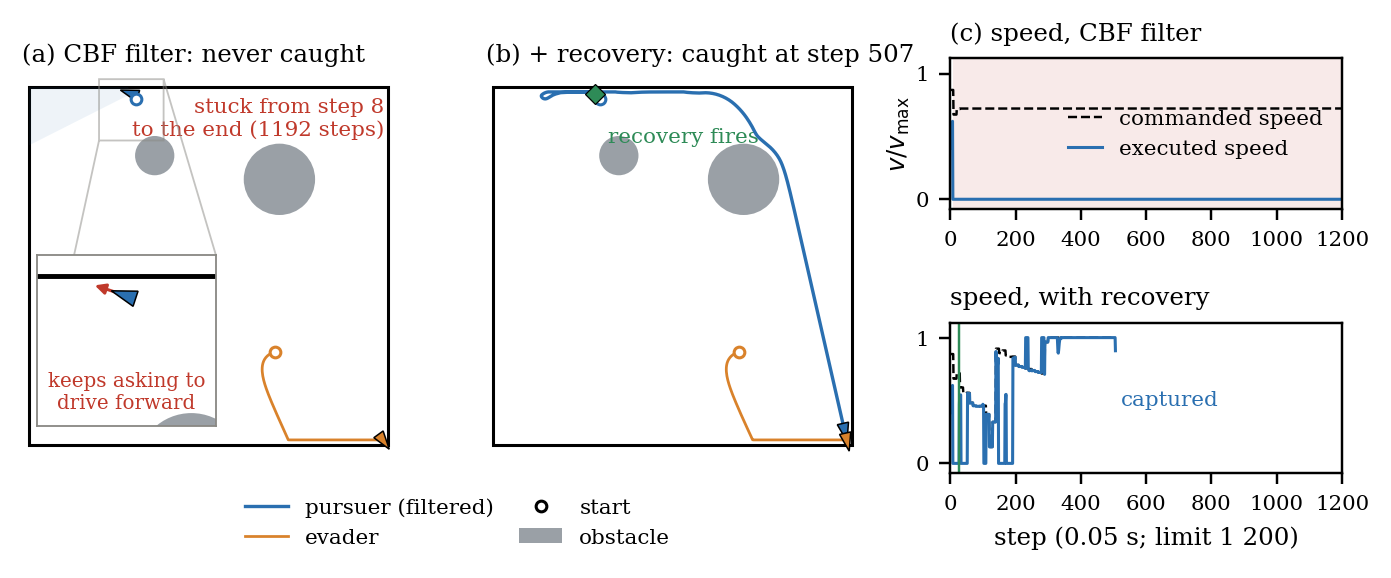
\includegraphics[width=\linewidth]{R0_game}
\caption{The failure in one episode (Experiment~7, policy \Free\ against the greedy evader, seed 1\,740\,044). (a)~With the CBF filter, the pursuer (blue) faces the top wall from step~8; its learned search head asks to drive forward (inset), the filter executes a standstill, and the request repeats for the remaining 1\,192 steps. The evader (orange) waits in a corner. (b)~The same episode with the recovery of Section~\ref{sec:recovery} at $N = 20$: it fires seven times, the pursuer turns away from the wall and captures at step 507. (c)~Commanded and executed speed; the shaded band is the stall. Zero collisions in both runs. The replay reproduces the archived outcome of both runs.}
\label{fig:game}
\end{figure}

\paragraph{The pursuer's controller.} The pursuer is a learning-enabled controller with two parts (Figure~\ref{fig:loop}). A scripted \emph{intercept law} acts whenever it has something to do: while the evader is visible it drives at full speed and steers toward it, and it remembers where it last saw it; while the evader is not visible it drives toward that remembered point until it is within \SI{0.5}{m}. Only then does a learned \emph{search head}, a PPO policy, choose a command, which is held for 10 steps or until the evader comes into view. The law therefore carries one piece of memory, the remembered point, which does not change while the evader stays out of view; the head has no memory. We call one head command and the law steps that follow it a \emph{decision}: it is one transition for the learner and lasts about 16 steps on average in training.

\begin{figure}[t]
\centering
\resizebox{0.74\linewidth}{!}{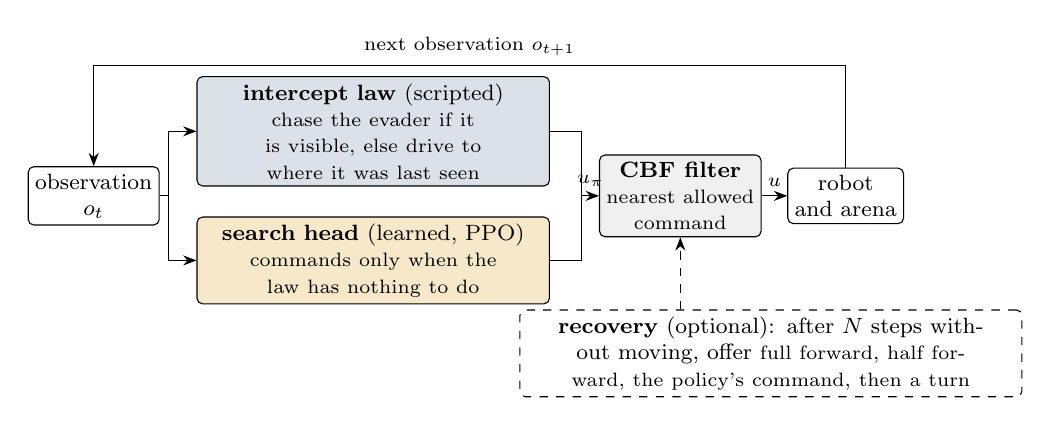
\begin{tikzpicture}[font=\footnotesize, >=Stealth,
  box/.style={draw, rounded corners=2pt, align=center, inner sep=2.5pt, minimum height=7mm},
  law/.style={box, fill=lawc!18, text width=4.3cm}, head/.style={box, fill=headc!25, text width=4.3cm}, filt/.style={box, fill=gray!12}]
\node[box] (obs) at (0,0) {observation\\$o_t$};
\node[law] (law) at (3.55,0.82) {\textbf{intercept law} (scripted)\\{\scriptsize chase the evader if it is visible, else drive to where it was last seen}};
\node[head] (head) at (3.55,-0.82) {\textbf{search head} (learned, PPO)\\{\scriptsize commands only when the law has nothing to do}};
\node[filt] (cbf) at (7.45,0) {\textbf{CBF filter}\\{\scriptsize nearest allowed}\\{\scriptsize command}};
\node[box] (env) at (9.55,0) {robot\\and arena};
\node[box, dashed, text width=6.2cm] (rec) at (8.6,-2.0) {\textbf{recovery} (optional): after $N$ steps without moving, offer {\scriptsize full forward, half forward, the policy's command, then a turn}};
\coordinate (split) at (0.95,0);
\coordinate (join) at (6.2,0);
\draw (obs.east) -- (split);
\draw[->] (split) |- (law.west);
\draw[->] (split) |- (head.west);
\draw (law.east) -| (join);
\draw (head.east) -| (join);
\draw[->] (join) -- node[above, font=\scriptsize]{$u_\pi$} (cbf.west);
\draw[->] (cbf) -- node[above, font=\scriptsize]{$u$} (env);
\draw[->] (env.north) -- ++(0,1.3) -| node[pos=0.25, above, font=\scriptsize]{next observation $o_{t+1}$} (obs.north);
\draw[->, dashed] (rec.north -| cbf.south) -- (cbf.south);
\end{tikzpicture}
}
\caption{The closed loop. The intercept law commands whenever the evader is visible or a remembered point has not yet been reached; the learned head commands otherwise. Every command passes through the CBF filter. The optional recovery is a counter beside the filter that offers it a short list of candidate commands; every executed command is still the filter's output.}
\label{fig:loop}
\end{figure}

\paragraph{Observation and reward.} The head observes 11 numbers: its own position and heading; the evader's relative position and heading, set to zero when the evader is not visible, and a visibility flag; and the centres of the two obstacles in its own frame. Obstacle radii are not observed, and walls are seen only through the pursuer's own position. Policies trained behind the filter also observe three filter features: whether the filter changed the last command, the smallest clearance, and the number of consecutive stalled steps divided by 40, which stops growing at 80 steps. The \Obs\ policies observe two more numbers, the range of turn rates the filter would allow at zero speed. The reward is $+1$ for a capture and $-1$ for a timeout; policies trained behind the filter also pay $10^{-3}$ per stalled step. The discount $\gamma$ applies once per decision.

\paragraph{Policies.} Table~\ref{tab:policies} lists the six policies. The four families of three seeds each were trained from scratch behind the filter with the filter features and the stall penalty; \Obs\ adds the allowed-turn features, \Hor\ raises the discount to 0.999, \ObsHor\ does both. \Free\ and \Aware\ come from earlier experiments, each the best of its training seeds on an earlier evaluation: \Free\ is a policy deployed behind a filter it never saw, and \Aware\ is \Base's recipe trained twice as long. All policies are frozen before evaluation; PPO settings are in the supplement.

\begin{table}[t]
\centering\footnotesize
\caption{The six policies. All use the same intercept law; they differ in the learned search head.}
\label{tab:policies}
\setlength{\tabcolsep}{4pt}
\begin{tabular}{@{}lllll@{}}
\toprule
Policy & Trained & Filter during training & Extra observation & Discount \\
\midrule
\Base\ (3 seeds) & 5\,M steps & CBF filter, stall penalty $10^{-3}$ & 3 filter features & 0.99 \\
\Obs\ (3 seeds) & 5\,M steps & same & + allowed-turn range & 0.99 \\
\Hor\ (3 seeds) & 5\,M steps & same & 3 filter features & 0.999 \\
\ObsHor\ (3 seeds) & 5\,M steps & same & + allowed-turn range & 0.999 \\
\Free\ & 10\,M steps & none & none & 0.99 \\
\Aware\ & 10\,M steps & CBF filter, stall penalty $10^{-3}$ & 3 filter features & 0.99 \\
\bottomrule
\end{tabular}
\end{table}

\paragraph{Filter.} The CBF filter checks a command by the exact one-step barrier condition on the next state (barrier rate 0.2, for a control point \SI{0.1}{m} ahead of the axle) and executes the allowed command nearest the requested one in the weighted distance $150\,(\Delta v)^2 + (\Delta\omega)^2$. It searches a set of candidate commands and accepts each by the exact test, with a relaxed and a backup tier for the rare state where no candidate passes. The exact test failed on one step in each 500-episode evaluation of Experiment~6, every stalled state sampled in Experiment~2 was on the exact tier, and the backup tier was never used. In every filtered evaluation of this paper the number of collision steps is zero. Experiment~8 uses a second filter, which accepts a command if a four-step rollout in the simulator followed by a stop step makes no contact.

\paragraph{Stalls.} A step is \emph{immobile} if the executed speed is at most $0.05\,\vmax$, and \emph{stalled} if it is immobile although the requested speed is at least $0.5\,\vmax$. A \emph{deadlock episode} contains at least 40 consecutive stalled steps (\SI{2}{s}). A stalled state is a \emph{trap at heading} if no allowed command at the current pose moves the pursuer, and a \emph{position trap} if this holds at every heading at that position.

\section{Why the stall is a fixed point}\label{sec:formal}

Let $s$ be the full state, $o(s)$ the head's observation, $u_\pi = (v_\pi, \omega_\pi)$ the controller's command and $\adm(s)$ the polytope of commands that satisfy the linearised barrier rows $a_j^\top u \le b_j(s)$ inside the box $[0,\vmax]\times[-\wmax,\wmax]$, with outward normals $a_j$. Let $W = \mathrm{diag}(150, 1)$ and $u^\star(s) = \arg\min_{u \in \adm(s)} (u - u_\pi)^\top W (u - u_\pi)$.

\begin{lemma}[Zero speed; after \citet{grover2023before}]\label{lem:kkt}
The projection $u^\star$ has zero speed if and only if some allowed command $\bar u = (0, \bar\omega) \in \adm(s)$ satisfies $W(u_\pi - \bar u) = \sum_{j \in J(\bar u)} \mu_j a_j$ with $\mu_j \ge 0$, where $J(\bar u)$ indexes the constraints active at $\bar u$, the box face $v \ge 0$ included; then $u^\star = \bar u$.
\end{lemma}

The condition is the KKT condition of the weighted projection, which has a unique solution; it is the single-robot, static-obstacle case of the force-equilibrium condition of \citet{grover2023before}. The implemented filter is a candidate search accepted by the exact nonlinear test. On the 262 stalled states of Experiment~2 it agrees with the projection in 98.1\% of states; in the remaining 1.9\% the projection would have moved the pursuer.

\begin{proposition}[Absorbing stall]\label{prop:fixed}
Suppose that at state $s$ (i) the filter executes $u = (0, 0)$, (ii) the evader stays out of view, or stays visible at a fixed relative position, and (iii) the commanding part's internal state is unchanged: the law's remembered point (which updates only on sight of the evader) or the head's held command. Then the pursuer's pose and the observation are unchanged except for the filter's stall counter, which stops changing after 80 steps. From then on $u_\pi$, $u$ and the pursuer's pose are constant until the evader enters, leaves or moves within the field of view.
\end{proposition}

\begin{proof}[Proof sketch]
By (i) the pose does not change. Every component of $o(s)$ is a function of the pose, of the evader's relative state if visible, and of the filter features. By (ii) the evader term is constant, and the stall counter saturates. By (iii) the commanding part maps the same input to the same command, and the filter maps the same command at the same pose to the same output.
\end{proof}

Lemma~\ref{lem:kkt} is known; Proposition~\ref{prop:fixed} is what the controller contributes. Condition~(i) is a property of the pair (command, filter), not of the position: at a trap at heading a turn would free the pursuer, but the controller never asks for one. Filter features in the observation change the fixed point's input, not its existence, and a policy that has learned not to ask for speed reaches the same standstill (Section~\ref{sec:dissociations}).

\paragraph{The recovery.}\label{sec:recovery} After $N$ consecutive immobile steps, the recovery passes the candidates $(\vmax, 0)$, $(\tfrac12\vmax, 0)$, the controller's command, $(0, \wmax)$ and $(0, -\wmax)$ through the filter in that order and executes the first whose filtered speed exceeds $0.05\,\vmax$. If none moves, it executes the larger filtered rotation if that exceeds \SI{0.1}{rad/s}. The counter resets on any step with motion.

\begin{proposition}[Recovery]\label{prop:recovery}
(a)~Every executed command is an output of the base filter at the current state, so the recovery inherits the filter's safety guarantee unchanged. (b)~Suppose (H1) the position is not a position trap; (H2) at every heading on the way to a freeing heading the filter allows a rotation of at least $\tfrac12\wmax$ in the same direction; and (H3) at the freeing heading the forward candidate moves the pursuer at more than $0.05\,\vmax$. Then the pursuer is displaced by \SI{0.10}{m} within $N + T_{\mathrm{turn}} + 40$ steps, where $T_{\mathrm{turn}}$ is one full turn (45 steps at $\wmax$, 89 at $\tfrac12\wmax$) and 40 steps cover \SI{0.10}{m} at the immobility threshold. (c)~No liveness guarantee is claimed: nothing excludes a stall--recover--stall cycle, which we measure.
\end{proposition}

Part~(a) holds by construction. Part~(b) follows because a rotation is executed at every recovery step on which no forward candidate moves, so the heading sweeps until the forward candidate passes. Its hypotheses are checked, not assumed: H1 held at all 262 stalled states of Experiment~2 and a rotation of at least $\tfrac12\wmax$ was allowed at every one; H2 and H3 along the whole turn are not checked. Experiment~7 tested the stronger pre-registered bound $N + 45$.

\section{Experiments}\label{sec:experiments}

\paragraph{Protocol.} Every experiment was registered before any of its numbers existed: hypotheses, pass bars, decision rules, and the sentence to write if a hypothesis failed. Code was frozen at a commit. Compared conditions use the same evaluation seeds (\emph{paired}), drawn from a stream not used in training. Most comparisons use 500 paired episodes and the exact two-sided binomial test on the discordant pairs at $p < 0.05$; intervals are 95\% Newcombe paired intervals. Each experiment names its primary hypotheses, without multiplicity correction; with 500 pairs the smallest detectable difference in capture is about 0.05--0.08, so smaller effects are fragile. Shared conditions must reproduce earlier records exactly, designated episodes are watched before any summary, and nothing is re-run after its number exists. Supplement Table~S1 lists the ten experiments with their registered verdicts; each verdict is also stated below, failures included. Evaluations use three evaders: greedy, wall-hugging and the learned attacker.


\subsection{The cost of the filter}\label{sec:cost}

In Experiment~1 the policy \Free\ captured the greedy evader in 0.728 of 500 episodes without the filter and in 0.396 with it (difference $-0.33$, interval $[-0.375, -0.289]$, $p = 3\times10^{-44}$); 0.540 of the filtered episodes were deadlock episodes. The registered bar for three retrained remedies was the filtered capture of the scripted pursuer that \Free\ was first compared with, 0.426. A stall penalty alone did not clear it (0.426, 0.464, 0.436 on three seeds). Adding the filter features did (0.522, 0.512, 0.544; $p \le 8\times10^{-4}$) and still left 0.11--0.30 of episodes in deadlock. The arm with both, which produced \Aware, reached 0.564, 0.550 and 0.444.

\subsection{What is stuck}\label{sec:stuck}

\begin{figure}[t]
\centering
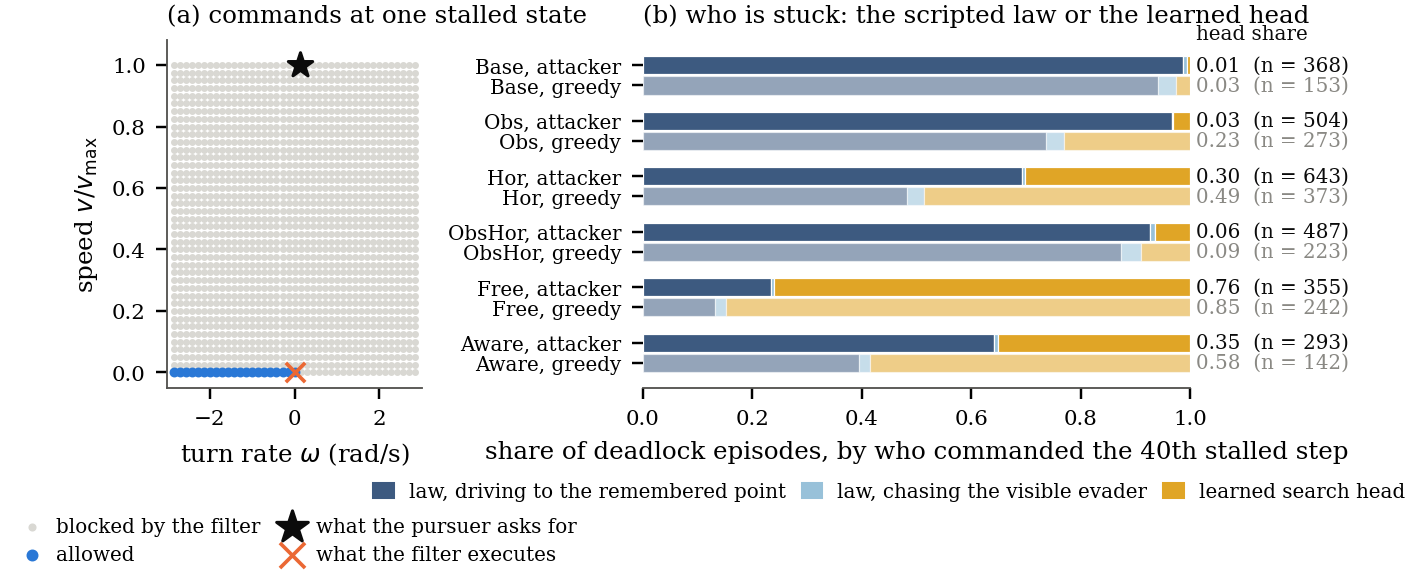
\includegraphics[width=\linewidth]{R2_stall}
\caption{(a)~Experiment~2: the commands the CBF filter allows at one archived stalled state (\Base\ seed 2): only standstill and turning. The policy asks for full speed; the filter executes zero. (b)~Experiment~3: for each deadlock episode, the part of the controller that commanded the 40th stalled step, against the learned attacker (dark) and the greedy evader (light); right, the learned head's share and the number of deadlock episodes.}
\label{fig:stall}
\end{figure}

\paragraph{Geometry (Experiment 2).} We sampled stalled states of four policies against the learned attacker, 100 episodes each, and tested every command on a grid at each state (Figure~\ref{fig:stall}a). All 262 stalled states are on the exact tier. In 98.1\% no allowed command moves the pursuer at its current heading. None is a position trap: at every one, another heading allows motion and a rotation of at least $\tfrac12\wmax$ is allowed. The registered bar for agreement between the filter and the exact projection was 99\%, and the measured 98.1\% missed it. A registered prediction that sampling noise would end the stall after a geometric waiting time failed. Deadlock with sampled actions was 0.42, 0.24, 0.29 and 0.57, against 0.38, 0.20, 0.21 and 0.55 with deterministic actions. The stall survives exploration.

\paragraph{Who commands the stall (Experiment 3).} The records behind the headline numbers carry no information about which part of the controller acted, so we replayed 40 archived evaluations: the four families against all three evaders, and \Free\ and \Aware\ against the attacker and the greedy evader. All 20\,000 replayed episodes reproduced the archive exactly. For each deadlock episode we recorded which part commanded the 40th stalled step. Figure~\ref{fig:stall}b shows the result. Against the learned attacker, the law driving to a remembered point owns 1\,747 of the four families' 2\,002 deadlock episodes, the learned head 243, and the law chasing a visible evader 12. The head's share is 0.005 for \Base, 0.03 for \Obs, 0.06 for \ObsHor\ and 0.30 for \Hor. For \Free\ the order reverses: the head owns 0.76 of the deadlock episodes against the attacker and 0.85 against the greedy evader; for \Aware\ it owns 0.35 and 0.58. All three registered predictions held. In the watched episodes, the law stalls against an obstacle between the pursuer and its remembered point, and the head stalls against a wall or in a corner, as in Figure~\ref{fig:game}.

\subsection{Why learning does not remove it}\label{sec:learning}

\paragraph{Law-owned stalls are outside learning.} A law stall happens inside one decision. The learner hands control to the law, the law drives into the obstacle, and the episode ends while the learner waits for its next turn. The learner can only change where it hands control to the law. That is consistent with Experiment~6, where every family without the recovery keeps deadlock between 0.19 and 0.61, and with the longer horizon of \Hor, which moves deadlock from the law to the head (head share 0.005 to 0.30) without reducing it.

\paragraph{Head-owned stalls carry a signal that is not used (Experiment 4).} We measured, on 383 stall entries of \Aware\ and its fine-tune, how much escaping is worth. Of the 97 escaped stalls, 0.299 were followed by a capture, against 0.042 of the 286 that were not. During a stall the world part of the observation does not change (median change 0.000) and the evader is visible in 3.4\% of stalled steps, so the input is frozen. Shortening the head's hold from 10 steps to 1 changed immobility by less than 0.05. The registered prediction was that the escape advantage is negligible: a difference in discounted return below 0.05 \emph{and} capture after escape below 0.15. It failed, because capture after escape is 0.299. The registered reading for this outcome is that the signal was there and learning missed it, a problem of optimisation, not of credit assignment.

\begin{remark}[The size of the signal]\label{rem:signal}
The registered analysis discounted per simulation step and found a return difference of 0.0092. The learner discounts per decision. A head stall advances 10 steps per decision. On that clock the difference is 0.29 at $\gamma = 0.99$, and $A_0\,\mathbb{E}[\gamma^{T}] = 0.18$, where $A_0 = 0.257$ is the capture advantage and $T$ is the number of decisions from the stall to the capture on the 29 captured escapes (346 steps on average). This is a post-hoc recomputation from the archived entries. It withdraws the explanation in our earlier analysis that the escape reward is discounted away.
\end{remark}

Why the head maps the stalled observation to the blocked command anyway is open. One candidate is aliasing: the observation contains neither the wall nor the obstacle's radius, so the stalled state resembles states where driving forward is right. Our one recurrent arm (Experiment~5) was confounded before its number existed, so memory is untested. \Free\ never saw the filter in training, so for it the question does not arise.

\paragraph{Learned remedies (Experiment 5).} Five learning-side remedies, three seeds each, and a scripted rotation-only recovery failed the registered primary metric, the immobile-step rate. The rotation-only recovery reached zero deadlock by spinning in place (414\,928 firings over 1\,500 episodes on one seed), although a straight command would have moved the pursuer at every sampled stalled pose; hence our recovery offers forward first.

\subsection{The recovery}\label{sec:recovery-results}

\begin{figure}[t]
\centering
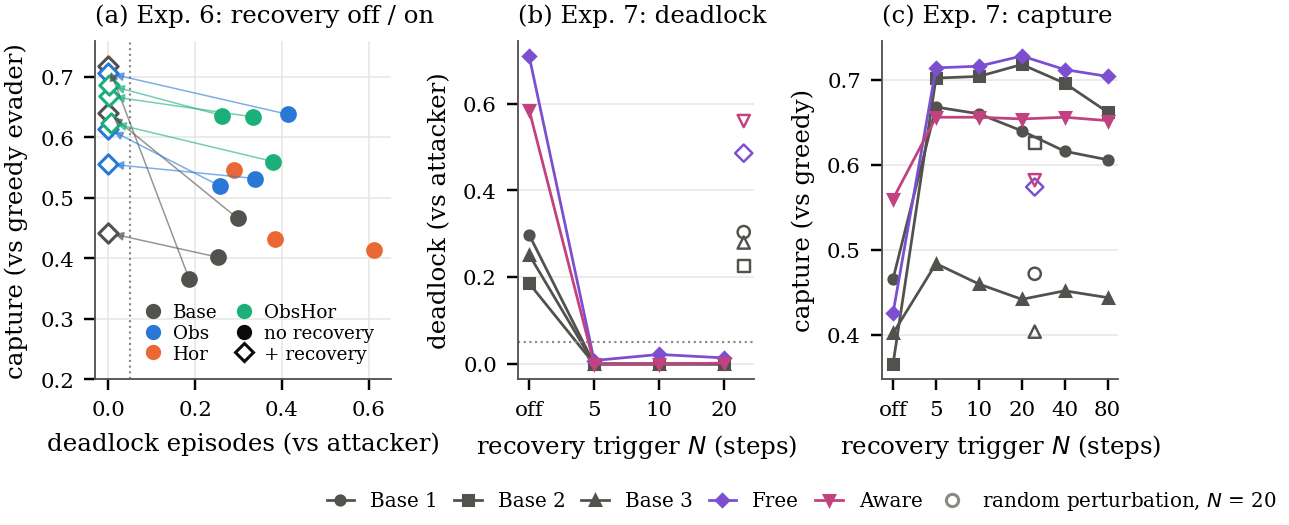
\includegraphics[width=\linewidth]{R4_recovery}
\caption{(a)~Experiment~6: deadlock against the learned attacker versus capture of the greedy evader, three seeds per family, without (filled) and with (open) the recovery at $N = 20$; arrows join each seed to itself. The dotted line is the registered deadlock bar 0.05. (b, c)~Experiment~7: deadlock and capture against the recovery trigger $N$ for five policies; open markers are the random-perturbation baseline at $N = 20$. Deadlock is drawn for $N \le 20$ only: for $N \ge 40$ the 40-step deadlock count includes the recovery's own wait, and longer-run counts are given in the text.}
\label{fig:recovery}
\end{figure}

\paragraph{Across families (Experiment 6).} Against the learned attacker, \Base's deadlock rate is 0.298, 0.186 and 0.252 on its three seeds. With the recovery at $N = 20$ it is 0.000 on the three \Base\ and three \Obs\ seeds and 0.006, 0.002 and 0.002 on the three \ObsHor\ seeds; the registered bar was 0.05 (Figure~\ref{fig:recovery}a). Capture of the greedy evader rises on nine of nine seeds: \Base\ from 0.466, 0.366, 0.402 to 0.640, 0.718, 0.442 (differences $+0.17$ $[+0.14, +0.21]$, $+0.35$ $[+0.31, +0.39]$, $+0.04$ $[+0.02, +0.06]$). The learned families without recovery raise capture too (\Obs\ 0.532, 0.520, 0.638; \Hor\ 0.546, 0.432, 0.414; \ObsHor\ 0.560, 0.634, 0.636) and keep deadlock between 0.26 and 0.61. Learning changes how often the recovery is needed: over 1\,500 episodes it fires 13\,035, 152\,675 and 27\,974 times for the \Base\ seeds and 35\,755, 363 and 513 times for the \ObsHor\ seeds, for similar capture.

\paragraph{The trigger $N$ and a random baseline (Experiment 7).} We swept $N \in \{5, 10, 20, 40, 80\}$ on \Base, \Free\ and \Aware\ (Figure~\ref{fig:recovery}b,c). Capture of the greedy evader is significantly above the plain filter at every $N$ on all five policies. For $N \le 20$, deadlock against the attacker is at most 0.022 on every policy, against 0.186--0.710 with the plain filter. For $N = 40$ and 80, stalls of at least $2N$ steps occur in at most 0.020 of episodes, against 0.176--0.682 plain. For \Free, capture rises from 0.426 to 0.728 ($+0.30$ $[+0.26, +0.34]$) and the immobile-step rate falls from 0.594 to 0.071; for \Aware, capture rises from 0.560 to 0.654 ($+0.09$ $[+0.07, +0.12]$). Across all $N$ and policies, the median time from a trigger to a \SI{0.10}{m} displacement is 4--10 steps. Within the registered bound $N + 45$ fall 97.8\% of 10\,475 triggers at $N = 20$; the registered per-evaluation bar of 95\% failed for \Base\ seed~3 (94.5\% and 92.3\%). The cost is cycling: at $N = 20$ between 8 and 56\% of recovery engagements end in another stall within 40 steps, while the immobile-step rate stays between 0.023 and 0.101.

The random baseline, the usual way to break a deadlock, draws up to eight commands from the command box after 20 still steps and executes the first whose filtered version moves the pursuer. We registered that it would clear the deadlock at a cost in capture. It cleared it on none of five policies (deadlock 0.304, 0.226, 0.280, 0.486, 0.560 against 0.298, 0.186, 0.252, 0.710, 0.586 plain), and the recovery captured more on all five. At a trap at heading no command moves the pursuer (Figure~\ref{fig:stall}a), so a baseline that executes only moving commands never turns, whereas 5--89\% of the recovery's firings are turns. The recovery's contribution is the turn, not the counter; a baseline that also accepts turns was not run.

\paragraph{A second filter (Experiment 8).} Under the predictive filter, deadlock against the attacker is 0.104, 0.036, 0.046 and 0.468 for the three \Base\ seeds and \Aware, against 0.298, 0.186, 0.252 and 0.586 under the CBF filter. The registered bar, deadlock of at least 0.05 on three of four policies, was met on two. The stall exists under the second filter but is weaker at this horizon; this filter is also less conservative, with no barrier-rate contraction, so the difference cannot be attributed to the filter's construction alone. With the recovery composed onto it, every candidate is judged by the predictive test. Deadlock falls to 0.000, 0.000, 0.002 and 0.014, and capture rises on four of four policies (0.468 to 0.628, 0.454 to 0.702, 0.396 to 0.432, 0.554 to 0.668; all $p < 0.05$).

\section{Stall metrics can improve while the task fails}\label{sec:dissociations}


Two penalties made a stall metric better and the task worse (supplement, Figure~S2). In Experiment~5, a family trained with a stall penalty ten times larger than the others' lowers its stalled-step rate (0.143--0.249 to 0.093--0.158), while its immobile-step rate rises (0.436--0.448 to 0.633--0.833) and its capture falls (0.384--0.478 to 0.204--0.348). It learns to stop asking to move: the requested speed itself becomes zero, and the standstill of Proposition~\ref{prop:fixed} is reached without a blocked request.

Experiment~9 used the penalty of \citet{pizarro2025filtering} on the size of the filter's correction, in unsquared normalised form. In their quadrotor tracking task it raised return; there, standing still is never locally optimal. Here, in the dense-reward variant, capture falls on three of three seeds (0.442, 0.480, 0.528 to 0.338, 0.300, 0.212; pooled $p = 3.6\times10^{-51}$), zero-speed requests rise (0.07, 0.16, 0.00 to 0.37, 0.78, 0.80), and deadlock improves in nine of nine evaluations. The registered prediction that the penalty helps under the dense reward and hurts under the sparse one failed: it never raised pooled capture (sparse 0.535 with and without; the other dense variant 0.555 to 0.535, $p = 0.13$). The penalty was also charged for the law's corrections, a registered confound.

In Experiment~10 (supplement), an obstacle-avoiding planner in place of the intercept law of a fully scripted pursuer cut law stalls from 0.13--0.37 of episodes to at most 0.008, while capture moved by $+0.026$, $-0.018$, $-0.022$. Report the task, the immobile-step rate and the stalled-step rate separately, and the firing count for any recovery.

\section{Discussion and limitations}\label{sec:discussion}

\paragraph{Scope.} One game, one robot model, static obstacles, two filters, six policies, three seeds per family. Moving obstacles or other agents would break the frozen input of Proposition~\ref{prop:fixed} and may shorten the stall. The head's share of stalls ranged from 0.005 to 0.85 with training, so claims about learned policies in general need that share measured; memory is untested.

\paragraph{The recovery} costs cycles, misses the stronger bound on 2.2\% of triggers, fires three orders of magnitude more for some policies than others, and offers no liveness guarantee. Its one design choice, offering a turn, is the one the geometry of Experiment~2 asks for.

\paragraph{How the failure was found.} Fifteen earlier specifications passed their bars while measuring this artefact; a person watching the animated episodes found it (1\,085 consecutive blocked requests in one episode). Watching designated episodes is now a gate in our protocol. In practice: keep the filter, add the counter, log its firings, watch the episodes.

\section{Conclusion}\label{sec:conclusion}

A minimal-intervention safety filter in front of a learning-enabled controller can create a fixed point at which the guarantee holds, collisions are zero and the task fails. The stall is a trap of the command, not of the position: a turn would free it, and neither part of the controller asks for one. The scripted part has no learner in its loop; the learned part has a reward signal for escaping and does not use it. A counter that offers the filter a forward and a turning command removes the stall without touching the guarantee. The failure is cheap to remove and easy to miss.

\paragraph{Reproducibility.} The environment, filters, policies, pre-registrations, frozen commits, per-episode records and rendered episodes of every experiment are released at [repository URL], with a map from the names used here to the repository's identifiers.

\subsection*{Generative AI Use}

Generative AI tools were used for methodology drafting, coding and experimental implementation, literature search, and writing and editing. The authors reviewed and verified all AI-assisted content and take responsibility for the final content of the paper.

\bibliography{references}

\end{document}
